% 第3章第3节：全源最短路（全源最短路问题；Floyd--Warshall算法；Johnson算法；方法比较与结果检验）。

\section{全源最短路}
\label{sec:all-pairs-shortest-paths}

在交通路网规划、通信路由表预计算以及图结构分析（如计算图的直径、中心性与距离核）中，我们往往需要同时获知图中任意两个顶点之间的最短路距离与路线。面对这一全源需求，第~\ref{sec:apsp-problem}小节先定义全源距离矩阵与前驱矩阵，并分析为何直接把第~\ref{sec:single-source-shortest-paths}节的单源算法重复运行$n$次会在含负权弧的图上遭遇复杂度瓶颈。随后分别建立两条经典路线：第~\ref{sec:floyd-warshall}小节的Floyd--Warshall算法按允许经过的中间顶点编号逐层递推，对应$(\min,+)$热带半环上的矩阵消元；第~\ref{sec:johnson-algorithm}小节的Johnson算法引入顶点势函数对边权做差消元，借一次Bellman--Ford计算将负权弧全部转化为非负约化权，再运行$n$次Dijkstra算法。第~\ref{sec:apsp-comparison}小节对比全源求解路线并说明如何独立核验距离矩阵与前驱矩阵。

\subsection{全源最短路问题}
\label{sec:apsp-problem}

设有限有向图$\mathcal G=(V,E)$的顶点集编号为$V=\{1,2,\ldots,n\}$，有向弧数为$m=|E|$（与前文记号$a$一致，本节在复杂度对比中亦写作$m$），每条弧$u\to v$带有实数权值$w(u,v)\in\mathbb R$（即$\ell_{u,v}$）。由定义~\ref{def:graph-opt-shortest-path}，全源最短路问题要求输出所有有序顶点对$(u,v)\in V\times V$之间的最短距离矩阵$\bm D=\bigl(d^*(u,v)\bigr)_{u,v\in V}\in(\mathbb R\cup\{\pm\infty\})^{n\times n}$，以及用于恢复各条最短路的前驱矩阵$\bm\Pi=\bigl(\pi(u,v)\bigr)_{u,v\in V}$。其中$\pi(u,v)$记录从$u$到$v$的某条最短路上终点$v$的直接前驱顶点（当$u=v$或$v$从$u$不可达时置为空$\mathrm{NIL}$）。

当图中不存在负环时，每个可达顶点对的距离$d^*(u,v)$都是有限实数，且前驱矩阵$\bm\Pi$的第$u$行恰好编码了一棵以$u$为根的最短路树：从终点$v$出发，依次沿$v\gets\pi(u,v)$回溯直至回到$u$，反转后即得一条从$u$到$v$的最短路。若图中存在负环，能够经过某负环从$u$到达$v$的顶点对距离为$-\infty$；实际应用中通常要求算法在存在负环时直接检测并报告该负环。

为什么不直接把全源最短路归结为$n$次独立的单源最短路查询？这取决于边权符号与图的稠密程度。当所有边权非负（$w(u,v)\geq0$）时，以每个顶点$u\in V$为源点各运行一次Dijkstra算法即可求解：采用二叉堆实现时单次耗时$O((n+m)\log n)$，$n$次合计$O(n(n+m)\log n)$（若采用Fibonacci堆则为$O(nm+n^2\log n)$）；在$m=\Theta(n)$的稀疏图上其$O(n^2\log n)$开销比$n^2$个距离输出的规模多一个对数因子，而在$m=\Theta(n^2)$的稠密图上，用数组扫描版的Dijkstra算法运行$n$次也只需$O(n^3)$时间。

真正的瓶颈出现在\emph{含负权弧}的有向图中。由于Dijkstra算法在存在负权弧时会因过早锁定顶点而失效（图~\ref{fig:graph-opt-dijkstra-counterexample}），可以改用Bellman--Ford算法；计入初始化，其时间上界为$O(n+nm)$。将Bellman--Ford算法简单重复$n$次，总时间复杂度达到$O(n^2+n^2m)$；当图是边数$m=\Theta(n^2)$的稠密图时，这一开销退化到$O(n^4)$。

为了突破$O(n^2+n^2m)$的瓶颈，图论中发展出两条截然不同的经典路线。

第一条路线面向稠密图与矩阵计算：既然所有单源查询共享同一张图，与其按边数一步步延长路径，不如按顶点编号$1,2,\ldots,n$依次开放允许充当中转站的中间顶点，用三重循环在$\Theta(n^3)$时间内完成全局动态规划，这就是第~\ref{sec:floyd-warshall}小节的Floyd--Warshall算法。

第二条路线面向含负边的稀疏图：既然负边是阻碍使用Dijkstra算法的唯一障碍，就先跑\emph{一次}Bellman--Ford算出每个顶点的势函数，利用路径上的裂项相消将所有弧权转化为非负权，随后再跑$n$次Dijkstra算法，把总时间从$O(n^2+n^2m)$降到$O(nm+n^2\log n)$，这就是第~\ref{sec:johnson-algorithm}小节的Johnson算法。

\subsection{Floyd--Warshall算法}
\label{sec:floyd-warshall}

\subsubsection{问题与思路}

在一般有向图上用动态规划求全源最短路，首先面临的问题是“按什么规模参数归纳”。第~\ref{sec:graph-opt-bellman-ford}小节的Bellman--Ford算法按路径包含的\emph{弧数}归纳：若记$L^{(r)}(i,j)$为从$i$到$j$至多含$r$条弧的最短路长度，则每增加一条弧，都需要枚举倒数第二个顶点$q\in\{1,\ldots,n\}$，计算$L^{(r)}(i,j)=\min\{L^{(r-1)}(i,j),\min_{q:q\to j}\{L^{(r-1)}(i,q)+w(q,j)\}\}$；第一项保留使用更少弧的路线。这种每次枚举一跳中转点的更新需要$O(n^3)$时间；若一步步递推到$r=n-1$，总时间仍需$O(n^4)$，即使借用矩阵幂的倍增技巧（依次计算$r=1,2,4,8,\ldots$）也仍需$O(n^3\log n)$时间，未能消去对数因子。

Floyd--Warshall算法的核心突破在于更换了动态规划的归纳维度：它不再限制路径经过的边数，而是限制路径上\emph{允许经过的中间顶点的编号范围}。具体而言，将顶点编号固定为$V=\{1,2,\ldots,n\}$。对任意路径$P=(v_0,v_1,\ldots,v_\ell)$，除起点$v_0$和终点$v_\ell$以外的内部顶点$v_1,\ldots,v_{\ell-1}$统称为该路径的\term{中间顶点}（intermediate vertex）；单条弧$i\to j$没有中间顶点，其内部顶点集为空集$\varnothing$。

先假设图中没有负环。对于每个阶段$k\in\{0,1,\ldots,n\}$，定义状态$d^{(k)}(i,j)$为：从$i$到$j$且\emph{所有中间顶点都取自集合$\{1,2,\ldots,k\}$}的全部路径的最小权值之和（若不存在这样的路径则记为$+\infty$）。当$k=0$时，中间顶点集为空，路径至多只能走单条直达弧；当$k$一路推进到$n$时，全部顶点都允许充当中间顶点，$d^{(n)}(i,j)$就恰好是全图上的真实最短距离$d^*(i,j)$。

如何从阶段$k-1$推进到阶段$k$？假设图中不含负环，考察从$i$到$j$、中间顶点均属于$\{1,\ldots,k\}$的一条最短简单路径$P$。面对新开放的编号$k$，这条最优路径$P$只有两种互斥的情形：第一种情形是$P$根本没有把顶点$k$当作中间顶点，此时$P$的所有中间顶点其实都落在$\{1,\ldots,k-1\}$内，其最优长度就是上一阶段的$d^{(k-1)}(i,j)$；第二种情形是$P$经过了中间顶点$k$，由于不含负环时简单路径不会重复访问顶点，$k$在$P$内部只出现唯一一次，并以$k$为界将$P$切分为从$i$到$k$的前半段与从$k$到$j$的后半段。这两段子路径自身不再包含$k$作为内部顶点，它们的中间顶点完全落在$\{1,\ldots,k-1\}$中，且各自必然是该限制下的最短路径，长度分别为$d^{(k-1)}(i,k)$与$d^{(k-1)}(k,j)$。在两种情形之间取最小，无需像按弧数递推那样耗费$O(n)$时间枚举跳点，只需做一次$O(1)$的二选一比较，便得到著名的\term{Floyd--Warshall算法}（Floyd--Warshall algorithm）状态转移方程：
\begin{equation}
  d^{(k)}(i,j) = \min\bigl\{d^{(k-1)}(i,j),\; d^{(k-1)}(i,k) + d^{(k-1)}(k,j)\bigr\},\qquad k=1,2,\ldots,n.
  \label{eq:floyd-warshall-recurrence}
\end{equation}
初始边界$d^{(0)}(i,j)$由直接相连的边权给出：对角线$d^{(0)}(i,i)=0$；当$i\neq j$且存在弧$i\to j$时$d^{(0)}(i,j)=w(i,j)$，否则为$+\infty$。

从代数的视角看，上述按弧数倍增和Floyd--Warshall递推都植根于\term{热带半环}（tropical semiring，亦称$(\min,+)$代数）。在集合$\mathbb R\cup\{+\infty\}$上，若将加法替换为取最小运算$a\oplus b=\min\{a,b\}$（零元为$+\infty$），将乘法替换为普通实数加法$a\otimes b=a+b$（单位元为$0$），则乘法对加法依然满足分配律：$a+(b\oplus c)=(a+b)\oplus(a+c)$。两个距离矩阵$\bm A,\bm B$在此半环上的\term{热带矩阵乘法}（tropical matrix multiplication）定义为
\begin{equation}
  (\bm A\otimes\bm B)_{i,j} = \min_{1\leq q\leq n}\bigl(A_{i,q}+B_{q,j}\bigr).
  \label{eq:tropical-matrix-mult}
\end{equation}
在这一代数语言下，取$L^{(0)}(i,i)=0$、$L^{(0)}(i,j)=+\infty$（$i\ne j$），并由$\bm D^{(0)}$的零对角线表示“不增加弧数”，按边数递推的矩阵序列恰好是初始距离矩阵的热带幂$\bm L^{(r)}=(\bm D^{(0)})^{\otimes r}$；而Floyd--Warshall递推式~\eqref{eq:floyd-warshall-recurrence}则与求矩阵传递闭包（Warshall算法）采用相同的逐顶点消元结构——每一步以第$k$行和第$k$列为枢轴，用秩一热带外积更新整个矩阵，从而以$n$次枢轴步取代了矩阵求幂，得到$\Theta(n^3)$的最坏时间界。

\subsubsection{算法实现}

在计算机实现中，我们无需开辟$n+1$个二维矩阵来分别存储$\bm D^{(0)},\ldots,\bm D^{(n)}$，而是可以直接在同一个$n\times n$距离数组$d(i,j)$和前驱数组$\pi(i,j)$上就地更新。当外层循环固定中间顶点$k$，且发现绕行$k$能够严格缩短从$i$到$j$的距离（即$d(i,k)+d(k,j)<d(i,j)$）时，除将$d(i,j)$改写为$d(i,k)+d(k,j)$外，还应同步更新终点$j$的前驱：由于新路线后半段沿用的是从$k$到$j$的最短路，在这条路上$j$的直接前驱正是从$k$到$j$路径上的最后一步$\pi(k,j)$，因此前驱更新规则为$\pi(i,j)\gets\pi(k,j)$。

含负环时，有限次递推得到的标签不能解释为允许任意重复顶点的最短闭行走长度，因为这一长度可能为$-\infty$。不过，每个有限标签仍对应某条实际行走的成本；因此$d(i,i)<0$表明存在经过$i$的负闭行走，该闭行走必包含负环，但负环未必经过$i$。反过来，若存在负环，递推最终会使至少一个对角标签变负，故检查主对角线即可检测负环。

\begin{algorithm}[Floyd--Warshall全源最短路算法]
\label{alg:floyd-warshall}
输入：有向加权图$\mathcal G=(V,E,w)$，顶点集$V=\{1,\ldots,n\}$。输出：全源最短距离矩阵$\bm D=(d(i,j))$与前驱矩阵$\bm\Pi=(\pi(i,j))$，或报告“存在负环”。
\begin{enumerate}
  \item 初始化矩阵：对所有$i,j\in\{1,\ldots,n\}$，若$i=j$则置$d(i,i)=0$、$\pi(i,i)=\mathrm{NIL}$；若$i\neq j$且$(i,j)\in E$，置$d(i,j)=w(i,j)$、$\pi(i,j)=i$；否则置$d(i,j)=+\infty$、$\pi(i,j)=\mathrm{NIL}$。
  \item 三重循环递推：按$k=1,2,\ldots,n$依次固定中间顶点：
    \begin{enumerate}
      \item 对每个起点$i=1,2,\ldots,n$，若$d(i,k)=+\infty$则跳过该$i$；
      \item 对每个终点$j=1,2,\ldots,n$，若$d(k,j)<+\infty$且$d(i,k)+d(k,j)<d(i,j)$，则令
      \[
        d(i,j)\gets d(i,k)+d(k,j),\qquad \pi(i,j)\gets \pi(k,j).
      \]
    \end{enumerate}
  \item 负环检查：对$i=1,2,\ldots,n$，若$d(i,i)<0$，报告“图中存在负环”并停止；否则返回$\bm D$与$\bm\Pi$。
\end{enumerate}
\end{algorithm}

\paragraph{四顶点含负边有向图算例}
下面用一张含负权弧但无负环的四顶点有向图逐步演示算法~\ref{alg:floyd-warshall}的执行过程。设顶点集$V=\{1,2,3,4\}$，共有六条有向弧，其权值分别为：
\[
  \begin{gathered}
    w(1,2)=-2,\quad w(1,3)=5,\quad w(2,3)=3,\\
    w(2,4)=2,\quad w(3,1)=4,\quad w(4,3)=-1.
  \end{gathered}
\]
图~\ref{fig:floyd-warshall-example}展示了该有向图的拓扑结构及算法在四个阶段中逐步解锁的最短路径，五个阶段的距离矩阵$\bm D^{(0)},\bm D^{(1)},\bm D^{(2)},\bm D^{(3)},\bm D^{(4)}$如下：
\[
  \begin{aligned}
    \bm D^{(0)} &= \begin{bmatrix}
      0 & -2 & 5 & +\infty \\
      +\infty & 0 & 3 & 2 \\
      4 & +\infty & 0 & +\infty \\
      +\infty & +\infty & -1 & 0
    \end{bmatrix}, &
    \bm D^{(1)} &= \begin{bmatrix}
      0 & -2 & 5 & +\infty \\
      +\infty & 0 & 3 & 2 \\
      4 & \mathbf{2} & 0 & +\infty \\
      +\infty & +\infty & -1 & 0
    \end{bmatrix}, \\[6pt]
    \bm D^{(2)} &= \begin{bmatrix}
      0 & -2 & \mathbf{1} & \mathbf{0} \\
      +\infty & 0 & 3 & 2 \\
      4 & 2 & 0 & \mathbf{4} \\
      +\infty & +\infty & -1 & 0
    \end{bmatrix}, &
    \bm D^{(3)} &= \begin{bmatrix}
      0 & -2 & 1 & 0 \\
      \mathbf{7} & 0 & 3 & 2 \\
      4 & 2 & 0 & 4 \\
      \mathbf{3} & \mathbf{1} & -1 & 0
    \end{bmatrix}, \\[6pt]
    \bm D^{(4)} &= \begin{bmatrix}
      0 & -2 & \mathbf{-1} & 0 \\
      \mathbf{5} & 0 & \mathbf{1} & 2 \\
      4 & 2 & 0 & 4 \\
      3 & 1 & -1 & 0
    \end{bmatrix}, &
    \bm\Pi^{(4)} &= \begin{bmatrix}
      \mathrm{NIL} & 1 & 4 & 2 \\
      3 & \mathrm{NIL} & 4 & 2 \\
      3 & 1 & \mathrm{NIL} & 2 \\
      3 & 1 & 4 & \mathrm{NIL}
    \end{bmatrix}.
  \end{aligned}
\]

对照矩阵观察每一轮枢轴顶点$k$带来的实质变化（矩阵中粗体数字表示本阶段刚刚改写的元素）。在$k=1$阶段，只有顶点$3$能直接进入$1$（$d^{(0)}(3,1)=4$），接上出弧$1\to 2$（权$-2$）后打通了路径$3\to 1\to 2$，使$d^{(1)}(3,2)$从$+\infty$降为$2$。在$k=2$阶段，以顶点$2$为中转站，顶点$1$借$1\to 2\to 3$将$d^{(2)}(1,3)$从直达的$5$改善为$-2+3=1$，借$1\to 2\to 4$将$d^{(2)}(1,4)$更新为$-2+2=0$；同时顶点$3$借上一轮刚打通的$3\to 1\to 2$再接$2\to 4$，得到三步路径$3\to 1\to 2\to 4$，使$d^{(2)}(3,4)=2+2=4$。在$k=3$阶段，原本没有出路回到左侧的顶点$2$和$4$分别经由$3$连接到$1$与$2$，填补了左下角的三处$+\infty$。到了最后的$k=4$阶段，负权弧$4\to 3$（权$-1$）发挥作用：从$1$到$3$改走三弧路径$1\to 2\to 4\to 3$，距离由$1$进一步降至$0+(-1)=-1$；从$2$到$3$改走$2\to 4\to 3$，距离由$3$降至$2+(-1)=1$；从$2$到$1$也随之改走$2\to 4\to 3\to 1$，距离由$7$降至$2+3=5$。终态主对角线全为$0$，确认无负环；由终态前驱矩阵$\bm\Pi^{(4)}$回溯$(1,3)$：$\pi(1,3)=4$、$\pi(1,4)=2$、$\pi(1,2)=1$，即恢复出最短路径$1\to 2\to 4\to 3$。

\begin{BookInlineFigure}
  \centering
  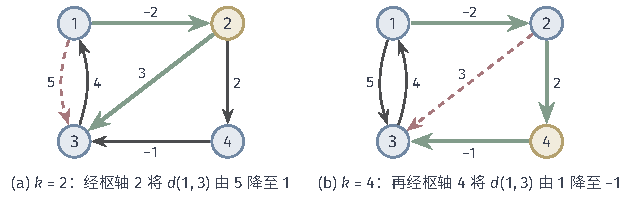
\includegraphics[width=107.184mm]{figures/03-graphs/02-combinatorial-optimization/tikz/floyd-warshall-example/figure.pdf}
  \caption{四顶点含负边有向图上Floyd--Warshall算法的逐层更新示例。黄色节点为当前阶段新开放的中间枢轴顶点$k$，绿色粗弧为当前阶段得到的$1\to 3$最短路线，红色虚弧为被替代的旧路线。(a) 阶段$k=2$开放顶点$2$后，绕行$1\to 2\to 3$（权和$-2+3=1$）替代直达弧$1\to 3$（权$5$）。(b) 阶段$k=4$开放顶点$4$后，绕行$1\to 2\to 4\to 3$（权和$-2+2-1=-1$）进一步替代$1\to 2\to 3$。}
  \label{fig:floyd-warshall-example}
\end{BookInlineFigure}

\subsubsection{算法分析}

\paragraph{正确性证明与就地更新次序}
我们先用对阶段$k$的数学归纳法证明递推式~\eqref{eq:floyd-warshall-recurrence}的正确性，再说明为何单数组就地更新不会破坏归纳假设。

\begin{theorem}[Floyd--Warshall算法的正确性]
\label{thm:floyd-warshall-correctness}
设有限有向加权图$\mathcal G=(V,E,w)$不含负环。对每个$k\in\{0,1,\ldots,n\}$及任意$i,j\in V$，由式~\eqref{eq:floyd-warshall-recurrence}递推得到的$d^{(k)}(i,j)$恰好等于从$i$到$j$且中间顶点均属于$\{1,\ldots,k\}$的最短路长度；特别地，算法~\ref{alg:floyd-warshall}结束时的$d(i,j)=d^{(n)}(i,j)=d^*(i,j)$。若图中存在负环，算法结束时必存在某个顶点$i$满足$d(i,i)<0$。
\end{theorem}

\begin{proof}
先设图中不含负环，对$k$进行归纳。当$k=0$时，中间顶点集$\{1,\ldots,k\}$为空集，从$i$到$j$不经过任何中间顶点的路径只有零步路径（$i=j$，成本$0$）或单条直达弧$i\to j$（成本$w(i,j)$），这与初始值$d^{(0)}(i,j)$的定义完全一致。

假设结论对$k-1$（$k\geq1$）成立。记$\mathcal P^{(k)}_{i,j}$为从$i$到$j$且中间顶点均属于$\{1,\ldots,k\}$的简单路径集合。由于不含负环，该限制下的最短行走可消去所有非负闭行走而化归为简单路径。一方面，$d^{(k-1)}(i,j)$对应一条中间顶点在$\{1,\ldots,k-1\}$内的路径，$d^{(k-1)}(i,k)+d^{(k-1)}(k,j)$对应将$i\leadsto k$与$k\leadsto j$两段中间顶点在$\{1,\ldots,k-1\}$内的路径在$k$处拼接所得的行走（其内部顶点属于$\{1,\ldots,k\}$），因此右端两项都是合法的候选成本，故$d^{(k)}(i,j)$不小于真实最优值。另一方面，任取一条达到该限制下最小成本的简单路径$P\in\mathcal P^{(k)}_{i,j}$：若$k$不是$P$的中间顶点，则$P\in\mathcal P^{(k-1)}_{i,j}$，由归纳假设其成本等于$d^{(k-1)}(i,j)$；若$k$是$P$的中间顶点，因$P$是简单路径，$k$在$P$内部仅出现一次，将$P$在$k$处切分为$P_1\in\mathcal P^{(k-1)}_{i,k}$与$P_2\in\mathcal P^{(k-1)}_{k,j}$，由归纳假设$w(P)=w(P_1)+w(P_2)\geq d^{(k-1)}(i,k)+d^{(k-1)}(k,j)$。综合两方面，式~\eqref{eq:floyd-warshall-recurrence}在阶段$k$精确成立。取$k=n$即得$d^{(n)}(i,j)=d^*(i,j)$。

再说明为何算法~\ref{alg:floyd-warshall}省略上标$(k)$、在单个二维数组$d(i,j)$上就地更新时结果完全不变。在第$k$轮内层循环中，更新$d(i,j)$读取的是同一轮中的$d(i,k)$和$d(k,j)$。注意当$j=k$时，候选值为$d^{(k-1)}(i,k)+d^{(k-1)}(k,k)$；在无负环假设下$d^{(k-1)}(k,k)=0$，故$d^{(k)}(i,k)=\min\{d^{(k-1)}(i,k),\,d^{(k-1)}(i,k)+0\}=d^{(k-1)}(i,k)$，同理$d^{(k)}(k,j)=d^{(k-1)}(k,j)$。也就是说，在第$k$轮迭代中，第$k$列元素$d(\cdot,k)$与第$k$行元素$d(k,\cdot)$的值根本不会改变。因此在更新任意位置$(i,j)$时，无论$(i,k)$或$(k,j)$在本轮中是先于$(i,j)$扫描还是后于$(i,j)$扫描，读取到的$d(i,k)$和$d(k,j)$都恒等于上一轮结束时的$d^{(k-1)}(i,k)$和$d^{(k-1)}(k,j)$，不会发生同轮覆盖污染。

最后，即使存在负环，按最大内部顶点拆分一条简单路径并归纳，仍可证明：当其内部顶点均已开放时，距离标签不大于这条路径的成本；就地更新只会进一步降低标签。若图中存在简单负环$C$，取$C$上编号最大的顶点记为$k^*$，取$C$上另一顶点$i^*$。$C$从$i^*$经$k^*$回到$i^*$，除$k^*$外其余顶点编号均小于$k^*$，故在阶段$k^*-1$结束时已有$d^{(k^*-1)}(i^*,k^*)+d^{(k^*-1)}(k^*,i^*)\leq w(C)<0$，从而在第$k^*$轮更新后$d(i^*,i^*)<0$；此后标签只降不升，算法结束时必检测到$d(i^*,i^*)<0$。
\end{proof}

上述关于就地更新的分析同时解释了一个常见的实现陷阱：\emph{三重循环的嵌套次序必须是$k$在最外层、$i$与$j$在内层（$k\to i\to j$），绝不能把循环次序调换为$i\to j\to k$}。若将$i,j$放在外层而只在最内层遍历$k=1,\ldots,n$，那么当固定一对$(i,j)$尝试用$d(i,k)+d(k,j)$更新$d(i,j)$时，其它顶点对$(i,k)$或$(k,j)$若排在$(i,j)$之后，就还未经过中间顶点$1,\ldots,k-1$的松弛更新，从而漏掉了大量需要多跳中转的最短路径。例如在前面的四顶点算例中，最短路径$2\to 4\to 3\to 1$依次经过编号为$4$和$3$的中间顶点（编号递减）；若外层先固定$(i,j)=(2,1)$再令$k=1,2,3,4$单趟递增，当检查$k=3$时$d(2,3)$尚未借$k=4$从$3$降为$1$，而当检查$k=4$时$d(4,1)$在初始表中还是$+\infty$，最终算出的$d(2,1)$将停留在错误的$7$而非真实的$5$。只有把$k$放在最外层，才能保证在进入阶段$k$之前，\emph{所有}顶点对的$d^{(k-1)}(\cdot,\cdot)$都已经完整算出。

\paragraph{时间与空间复杂度}
算法~\ref{alg:floyd-warshall}有三层至多运行$n$次的循环，最内层执行常数次运算，故最坏时间复杂度为$\Theta(n^3)$。本算法会跳过不可达的$i,k$组合，特定稀疏实例的实际工作量可能更少。距离矩阵与前驱矩阵各占$\Theta(n^2)$空间。规则的矩阵访问便于实现，但具体运行速度仍取决于数据布局、硬件与实现方式。

\subsection{Johnson算法}
\label{sec:johnson-algorithm}

\subsubsection{问题与思路}

当图是边数$m\ll n^2$的稀疏图（如道路网或大规模稀疏网络，$m=O(n)$）且含有负权弧时，Floyd--Warshall算法的$\Theta(n^3)$最坏时间上界可能高于利用稀疏性的算法。我们在第~\ref{sec:apsp-problem}小节看到，若能对每个源点运行一次Dijkstra算法，$n$次查询仅需$O(nm+n^2\log n)$时间；需要处理的障碍是图中的负权弧。于是自然产生这样一个问题：能否对图上每条弧的权值$w(u,v)$做一次变换，生成一组全新的\emph{非负}弧权$\tilde w(u,v)\geq0$，并且保证新权值下的最短路径与原权值下的最短路径完全相同？

初学者最容易想到的一种朴素方案是“全局平移”：找出全图最负的边权$-C$（其中$C>0$），把每一条弧的权值统一加上常数$C$，令$w'(u,v)=w(u,v)+C\geq0$。遗憾的是，这种平移会\emph{改变最短路径本身}。原因在于，一条包含$k$条弧的路径$P$，在新权值下的总长度会变成$w'(P)=w(P)+kC$：经过的弧数$k$越多，被额外追加的惩罚$kC$就越大。例如从$s$到$t$有一条直达弧（权$2$，含$1$条弧）和一条经过两个中转点的三弧路线（各段权$2,2,-3$，总权$1$，含$3$条弧），原本三弧路线更短（$1<2$）；若为消去$-3$而给每条弧统一加上$C=3$，直达弧新权变为$2+3=5$，而三弧路线被加上了$3\times3=9$，新总权变成$1+9=10>5$，原本的最短路反而被误判为更长。

朴素平移之所以失败，是因为路径的附加量$kC$取决于路径的内部边数$k$。要想让连接同一对起点$s$和终点$t$的所有路径在变换后增加完全相同的常数（与路径内部经过多少条弧、走哪条路线无关），每条弧的改变量就必须在路径拼接时“首尾相消”。这正是引入\term{顶点势}（vertex potential，亦称势函数）的核心动机：为每个顶点$v\in V$赋予一个实数势$h(v)\in\mathbb R$，并将每条弧$(u,v)\in E$的\term{约化权}（reduced weight，在流网络中对应第~\ref{chap:min-cost-flow}章的约化费用）定义为
\begin{equation}
  \tilde w(u,v) = w(u,v) + h(u) - h(v).
  \label{eq:johnson-reduced-weight}
\end{equation}

考察任意一条从起点$s=v_0$到终点$t=v_k$的路径$P=(v_0,v_1,\ldots,v_k)$。将路径上各段弧的约化权相加，所有内部顶点$v_1,\ldots,v_{k-1}$的势函数一负一正恰好裂项相消（telescoping sum）：
\begin{equation}
  \begin{aligned}
    \tilde w(P) &= \sum_{r=1}^{k}\tilde w(v_{r-1},v_r)
    = \sum_{r=1}^{k}\bigl(w(v_{r-1},v_r) + h(v_{r-1}) - h(v_r)\bigr) \\
    &= \sum_{r=1}^{k}w(v_{r-1},v_r) + h(v_0) - h(v_k)
    = w(P) + h(s) - h(t).
  \end{aligned}
  \label{eq:johnson-telescoping}
\end{equation}
式~\eqref{eq:johnson-telescoping}表明：当固定起点$s$和终点$t$时，不管路径$P$中途绕了多少条边，它的新成本$\tilde w(P)$与原成本$w(P)$永远只相差一个仅依赖于端点$s,t$的固定常数$h(s)-h(t)$。因此，对于任意两组$s$--$t$路径$P_1,P_2$，有$\tilde w(P_1)\leq\tilde w(P_2)$当且仅当$w(P_1)\leq w(P_2)$；新权值$\tilde w$保持了所有顶点对之间的最短路径集合。更进一步，对任意闭行走（或有向环）$C$，因其起点与终点相同（$s=t$），首尾势差$h(s)-h(s)=0$也一并抵消，得到$\tilde w(C)=w(C)$，即势函数重赋权保持每个有向环的总权值不变。

现在只剩下最后一个关键问题：怎样挑选这组顶点势$h:V\to\mathbb R$，才能使全图每一条弧$(u,v)\in E$的约化权都满足非负条件$\tilde w(u,v)\geq0$？将式~\eqref{eq:johnson-reduced-weight}改写为不等式，我们需要对每条弧$(u,v)\in E$同时满足
\begin{equation}
  h(v) \leq h(u) + w(u,v).
  \label{eq:johnson-triangle-ineq}
\end{equation}
对照第~\ref{sec:graph-opt-sp-relaxation}小节的最短路最优性证书式~\eqref{eq:graph-opt-shortest-path-certificate}，式~\eqref{eq:johnson-triangle-ineq}正是单源最短路距离天然满足的三角不等式。只要原图$\mathcal G$不含负环，我们只需在原图外添置一个虚拟\emph{超级源点}$s_0\notin V$，并从$s_0$向原图每个顶点$v\in V$各连一条权值为$0$的有向弧$s_0\to v$（构成扩展图$\mathcal G'=(V\cup\{s_0\},E\cup\{(s_0,v):v\in V\})$）。由于$s_0$没有任何入弧，新增的弧不会创造出任何新的有向环，$\mathcal G'$与$\mathcal G$具有完全相同的有向环，且原图每个顶点$v$都从$s_0$一步可达（距离至多为$0$）。在扩展图$\mathcal G'$上以$s_0$为源点运行一次Bellman--Ford算法：若算法报告存在可达负环，则原图$\mathcal G$必含负环；否则，取每个顶点的势为从$s_0$出发的最短路距离
\begin{equation}
  h(v) = d^*_{\mathcal G'}(s_0,v)\in\mathbb R,\qquad\forall v\in V,
  \label{eq:johnson-potential-choice}
\end{equation}
由最短路距离的三角不等式立即保证对一切$(u,v)\in E$都有$h(v)\leq h(u)+w(u,v)$，从而$\tilde w(u,v)=w(u,v)+h(u)-h(v)\geq0$恒成立。这就是1977年由Donald B. Johnson提出的\term{Johnson算法}（Johnson's algorithm）。

\subsubsection{算法实现}

Johnson算法的完整流程分为三个阶段：第一阶段构造超级源点$s_0$并调用一次Bellman--Ford算法，同时完成负环检测与顶点势$h(v)$的计算；第二阶段遍历全部有向弧计算非负约化权$\tilde w(u,v)$；第三阶段在非负权图$(\mathcal G,\tilde w)$上依次以每个顶点$u\in V$为源点调用Dijkstra算法求出重赋权后的最短距离$\tilde d^*(u,v)$，最后利用逆变换$d^*(u,v)=\tilde d^*(u,v)-h(u)+h(v)$还原出原始权值下的真实全源最短距离矩阵。

\begin{algorithm}[Johnson全源最短路算法]
\label{alg:johnson-apsp}
输入：有向加权图$\mathcal G=(V,E,w)$。输出：全源最短距离矩阵$\bm D=(d^*(u,v))_{u,v\in V}$与前驱矩阵$\bm\Pi$，或报告“存在负环”。
\begin{enumerate}
  \item 构造扩展图与计算势函数：令$V'=V\cup\{s_0\}$，$E'=E\cup\{(s_0,v):v\in V\}$，对每个$v\in V$置$w(s_0,v)=0$。在$\mathcal G'=(V',E',w)$上以$s_0$为源点运行Bellman--Ford算法（算法~\ref{alg:graph-opt-bellman-ford}）。若检测到负环，报告“图中存在负环”并停止；否则对每个$v\in V$令$h(v)=d^*_{\mathcal G'}(s_0,v)$。
  \item 边权重赋权：对每条原图有向弧$(u,v)\in E$，计算非负约化权
  \[
    \tilde w(u,v) \gets w(u,v) + h(u) - h(v).
  \]
  \item 重复运行Dijkstra并还原距离：对每个源点$u\in V$：
    \begin{enumerate}
      \item 在非负加权图$(V,E,\tilde w)$上以$u$为源点运行Dijkstra算法（算法~\ref{alg:graph-opt-dijkstra}），得到距离向量$\tilde d^*(u,v)$与前驱$\pi(u,v)$（$\forall v\in V$）；
      \item 对每个终点$v\in V$，若$\tilde d^*(u,v)=+\infty$则置$d^*(u,v)=+\infty$，否则还原真实最短距离：
      \[
        d^*(u,v) \gets \tilde d^*(u,v) - h(u) + h(v).
      \]
    \end{enumerate}
  \item 返回距离矩阵$\bm D=(d^*(u,v))$与前驱矩阵$\bm\Pi=(\pi(u,v))$。
\end{enumerate}
\end{algorithm}

\paragraph{四顶点有向图算例的重赋权演示}
我们在与第~\ref{sec:floyd-warshall}小节完全相同的四顶点六弧有向图上演示算法~\ref{alg:johnson-apsp}（图~\ref{fig:johnson-reweighting}）。

第一步，引入超级源点$s_0$并连接四条零权弧$s_0\to 1,2,3,4$（图~\ref{fig:johnson-reweighting}a）。从$s_0$出发运行Bellman--Ford算法：到顶点$1$和$4$的最短路即零权直达弧，故$h(1)=0$、$h(4)=0$；到顶点$2$经由$s_0\to 1\to 2$取得最小成本$0+(-2)=-2$，故$h(2)=-2$；到顶点$3$经由$s_0\to 4\to 3$（或$s_0\to 1\to 2\to 4\to 3$）取得最小成本$0+(-1)=-1$，故$h(3)=-1$。所得顶点势向量为
\[
  \bigl(h(1),\,h(2),\,h(3),\,h(4)\bigr) = (0,\,-2,\,-1,\,0).
\]

第二步，按式~\eqref{eq:johnson-reduced-weight}逐条计算六条弧的约化权$\tilde w(u,v)=w(u,v)+h(u)-h(v)$（图~\ref{fig:johnson-reweighting}b）：
\[
  \begin{aligned}
    \tilde w(1,2) &= -2 + 0 - (-2) = 0, &\qquad \tilde w(1,3) &= 5 + 0 - (-1) = 6, \\
    \tilde w(2,3) &= 3 + (-2) - (-1) = 2, &\qquad \tilde w(2,4) &= 2 + (-2) - 0 = 0, \\
    \tilde w(3,1) &= 4 + (-1) - 0 = 3, &\qquad \tilde w(4,3) &= -1 + 0 - (-1) = 0.
  \end{aligned}
\]
可以看到，原本为负的弧$1\to 2$（权$-2$）和$4\to 3$（权$-1$），连同位于从$s_0$出发的最短路树上的弧$2\to 4$，在重赋权后约化权全部变为$0$（对应势不等式取等），其余三条弧的约化权分别为$6,2,3$，全图所有弧权均已非负。

第三步，在非负权图$(V,E,\tilde w)$上从每个顶点$u\in\{1,2,3,4\}$分别运行Dijkstra算法：
\begin{itemize}
  \item 以$u=1$为源点：沿零权路径$1\to 2\to 4\to 3$，Dijkstra算法算出到全部四个顶点的约化最短距离均为$\tilde d^*(1,\cdot)=(0,0,0,0)$。代入还原公式$d^*(1,v)=\tilde d^*(1,v)-h(1)+h(v)=0-0+h(v)$，立即恢复出第$1$行真实距离$(0,-2,-1,0)$。
  \item 以$u=2$为源点：沿$2\to 4\to 3$得$\tilde d^*(2,4)=\tilde d^*(2,3)=0$，再经$3\to 1$（约化权$3$）得$\tilde d^*(2,1)=3$，即$\tilde d^*(2,\cdot)=(3,0,0,0)$。减去$h(2)=-2$并加上各终点势$h(v)$，还原得第$2$行真实距离$(3+2+0,\,0+2-2,\,0+2-1,\,0+2+0)=(5,0,1,2)$。
  \item 以$u=3$和$u=4$为源点：同理分别由Dijkstra算出$\tilde d^*(3,\cdot)=(3,3,0,3)$与$\tilde d^*(4,\cdot)=(3,3,0,0)$，还原后得到第$3$行$(4,2,0,4)$与第$4$行$(3,1,-1,0)$。
\end{itemize}
本例四次Dijkstra还原出的距离矩阵与前小节的$\bm D^{(4)}$一致，前驱矩阵也可取为所列的$\bm\Pi^{(4)}$。一般存在多条等长最短路时，不同算法的前驱矩阵可以不同。

\begin{BookInlineFigure}
  \centering
  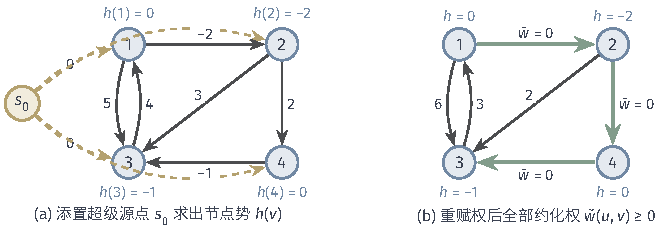
\includegraphics[width=112.843mm]{figures/03-graphs/02-combinatorial-optimization/tikz/johnson-reweighting/figure.pdf}
  \caption{Johnson算法在四顶点含负边有向图上的势函数重赋权过程。(a) 添置超级源点$s_0$（黄色）并向各点连零权虚线弧，运行一次Bellman--Ford得到顶点势$(h(1),h(2),h(3),h(4))=(0,-2,-1,0)$。(b) 按$\tilde w(u,v)=w(u,v)+h(u)-h(v)$重赋权后，原最短路树上的弧（绿色粗弧）约化权变为$0$，其余弧约化权为正数$6,2,3$，全图不含负权弧。}
  \label{fig:johnson-reweighting}
\end{BookInlineFigure}

\subsubsection{算法分析}

\paragraph{正确性与最优路径保持定理}
我们将前面的推导总结为如下定理。

\begin{theorem}[Johnson重赋权的非负性与最优路径保持]
\label{thm:johnson-correctness}
设有限有向加权图$\mathcal G=(V,E,w)$。
\begin{enumerate}
  \item 对任意给定的势函数$h:V\to\mathbb R$，由$\tilde w(u,v)=w(u,v)+h(u)-h(v)$定义的约化权保持所有顶点对之间的最短路径不变：一条$s$--$t$路径$P$在原权$w$下是最短路，当且仅当$P$在约化权$\tilde w$下是最短路；且有向环$C$满足$\tilde w(C)=w(C)$。
  \item 原图$\mathcal G$不含负环当且仅当扩展图$\mathcal G'$从超级源点$s_0$出发不含可达负环。此时取$h(v)=d^*_{\mathcal G'}(s_0,v)$均有限，且对每条弧$(u,v)\in E$均有$\tilde w(u,v)\geq0$，算法~\ref{alg:johnson-apsp}正确输出全源最短距离矩阵$\bm D$与前驱矩阵$\bm\Pi$。
\end{enumerate}
\end{theorem}

\begin{proof}
第1条由裂项恒等式~\eqref{eq:johnson-telescoping}直接给出：对固定端点$s,t$，任意$s$--$t$行走$W$满足$\tilde w(W)=w(W)+h(s)-h(t)$，两边对$W\in\mathcal W_{s,t}$取下确界即得$\tilde d^*(s,t)=d^*(s,t)+h(s)-h(t)$，且取到下确界的路径完全一致。闭行走满足$s=t$，故$\tilde w(C)=w(C)$。

下证第2条。因为$s_0$在$\mathcal G'$中入度为$0$，$\mathcal G'$中的任何有向环都不可能包含$s_0$，故$\mathcal G'$的有向环集合与$\mathcal G$完全相同；又因$s_0$有直达弧通向$V$中每个顶点，$\mathcal G$中任何负环在$\mathcal G'$中都从$s_0$可达。当无负环时，由于存在零权弧$s_0\to v$，有$-\infty<d^*_{\mathcal G'}(s_0,v)\leq0$，故$h(v)$必为有限实数。对任意$(u,v)\in E$，从$s_0$到$u$的最短路接上弧$u\to v$构成一条从$s_0$到$v$、成本为$h(u)+w(u,v)$的行走，由最短距离的下界性质得$h(v)\leq h(u)+w(u,v)$，移项即$\tilde w(u,v)=w(u,v)+h(u)-h(v)\geq0$。既然$\tilde w\geq0$，第三步中每次调用Dijkstra算法都能正确求出$\tilde d^*(u,v)$（定理~\ref{thm:graph-opt-dijkstra}），再经$d^*(u,v)=\tilde d^*(u,v)-h(u)+h(v)$还原即得原图的精确距离。
\end{proof}

\paragraph{复杂度分析与后续章节的联系}
我们来核算算法~\ref{alg:johnson-apsp}的三步开销：第一步在含$n+1$个顶点、$m+n$条弧的扩展图$\mathcal G'$上运行一次Bellman--Ford算法，耗时$O(n(n+m))=O(nm+n^2)$；第二步重赋权遍历全部$m$条弧，耗时$O(m)$；第三步运行$n$次Dijkstra算法，若采用Fibonacci堆实现，单次耗时$O(m+n\log n)$，$n$次共耗时$O(nm+n^2\log n)$（若采用普通二叉堆实现，则为$O(n(n+m)\log n)$），最后还原$n^2$个距离值耗时$O(n^2)$。因此，Johnson算法的总时间复杂度为
\begin{equation}
  T_{\mathrm{Johnson}}(n,m) = O(nm + n^2\log n)\quad\text{（二叉堆实现下为 }O(n(n+m)\log n)\text{）},
  \label{eq:johnson-complexity}
\end{equation}
除存储输出的$n\times n$矩阵外，工作空间仅为$O(n+m)$。在$m=O(n)$的稀疏图上，Johnson算法耗时$O(n^2\log n)$，比Floyd--Warshall算法的$\Theta(n^3)$具有更低的渐近时间上界。

值得特别指出的是，Johnson算法中“利用顶点势调整边权、依靠路径裂项相消保持目标差值不变”的思想，并非全源最短路独有的技巧，而是贯穿本部分后续章节的一条核心主线。在第~\ref{chap:bipartite-matching-assignment}章的带权指派问题中，可行标号与物品价格正是二部图上的顶点势；到了第~\ref{chap:min-cost-flow}章（最小费用流），式~\eqref{eq:johnson-reduced-weight}中的约化权在取$\pi=-h$的记号约定后，对应残量网络上的“约化费用”$\bar c_{i,j}=c_{i,j}-\pi_i+\pi_j$（式~\eqref{eq:graph-opt-reduced-cost}），而逐次最短路算法每轮借节点势把残量弧费用维持为非负、从而反复调用Dijkstra算法增广的做法，更是Johnson势函数重赋权在流网络上的直接延伸。

\subsection{方法比较与结果检验}
\label{sec:apsp-comparison}

求解全源最短路的四种主要方案——$n$次Bellman--Ford、$n$次Dijkstra、Floyd--Warshall算法与Johnson算法——在适用条件、数据结构依赖和渐近复杂度上各有侧重，表~\ref{tab:apsp-methods-comparison}将它们并列对比。

\begin{table}[!htb]
  \centering
  \begin{tabular}{@{}lllll@{}}
    \toprule
    方法 & 允许负权弧 & 负环检测 & 时间复杂度 & 典型适用场景 \\
    \midrule
    $n$次Dijkstra & 否（要求$w\geq0$） & 不适用 & $O(nm+n^2\log n)^*$ & 非负权稀疏图 \\
    $n$次Bellman--Ford & 是 & 支持 & $O(n^2+n^2m)$ & 仅作基准对照 \\
    Floyd--Warshall & 是 & 对角线$d(i,i)<0$ & $\Theta(n^3)$ & 稠密图、矩阵/小规模图 \\
    Johnson算法 & 是 & 超级源点BF检测 & $O(nm+n^2\log n)^*$ & 含负权弧的稀疏图 \\
    \bottomrule
  \end{tabular}
  \caption{全源最短路求解方法的比较（$n=|V|$为顶点数，$m=|E|$为有向弧数；带$^*$号为Fibonacci堆界，使用二叉堆时为$O(n(n+m)\log n)$，稠密图用数组扫描版Dijkstra为$O(n^3)$）。}
  \label{tab:apsp-methods-comparison}
\end{table}

选择算法时，先检查弧权条件和输出需求。非负权图可以逐源运行Dijkstra算法；含负权弧时，Floyd--Warshall与Johnson都可检测负环，在无负环时返回全源距离。稠密图上可比较Floyd--Warshall与数组版Dijkstra的立方时间实现，稀疏图上则可考虑Johnson。理论复杂度不能直接确定某个顶点数阈值下哪一种实现更快，具体选择还需结合存储与运行测量。

拿到一份无负环图上的全源最短路输出$(\bm D,\bm\Pi)$后，怎样不重跑算法而独立核对它的正确性？与第~\ref{sec:graph-opt-sssp-comparison}小节的单源检验一脉相承，核验分为“上界可达到”与“下界最优性”两步：
\begin{enumerate}
  \item 可达性见证（$d(u,v)\geq d^*(u,v)$）：对每个源点$u\in V$，检查$d(u,u)=0$，并对每个满足$d(u,v)<+\infty$且$v\neq u$的顶点$v$，验证前驱边$(\pi(u,v),v)\in E$、前驱链不形成有向环且满足等式
  \[
    d(u,v) = d\bigl(u,\pi(u,v)\bigr) + w\bigl(\pi(u,v),v\bigr).
  \]
  这保证沿着$\bm\Pi$的第$u$行回溯必能到达$u$，且该路径的真实弧长之和恰好等于$d(u,v)$。
  \item 逐弧三角不等式证书（$d(u,v)\leq d^*(u,v)$）：对每个源点$u\in V$与图中的每条有向弧$(x,y)\in E$，核对三角不等式
  \begin{equation}
    d(u,y) \leq d(u,x) + w(x,y).
    \label{eq:apsp-certificate}
  \end{equation}
  只要式~\eqref{eq:apsp-certificate}对所有$u\in V$和$(x,y)\in E$成立，沿任意$u\leadsto v$路径累加即证$d(u,v)\leq d^*(u,v)$。两步合在一起，仅需$O(n(n+m))$时间即可完成对全源最短路矩阵$(\bm D,\bm\Pi)$的完备检验。
\end{enumerate}
